\section{Code Examples} 
\label{sec:examples} 
All the examples are located in different sub-folders inside a folder
called {\ttf examples}, the examples can be compiled using the
general make file, {\ttf make examples}.
Some of the examples contain a Gnuplot script to plot the output file,
the text files with the values are also generated and can be plotted
with any other plotting tool.
In the following we present one by one the examples.


\subsection{Single Energy \textnormal{({\ttf examples/Single\_energy})}}
\label{sec:single}
This example illustrates the use of the simplified mode to compute the
propagation of the neutrinos for a single energy mode, notice that
this can not be accurate at high energies but is a good approximation
for many of the neutrinos oscillation cases.

In the following we will go though the different lines in the main
function of the example.

First we need to construct the nusquids object with some parameters,
in this case we put 3 neutrinos and tell that the particle is
neutrino({\ttf neutrino}).
\begin{lstlisting}[frame=leftline, numbers = left,breaklines=true, label = ex:sin1]
  nuSQUIDS nus(3,neutrino);
\end{lstlisting}

In the following function we set the value of the paramters, we put
the value for the mixing angles in radians, the value for the mass
square difference and a value for the CP face.
 
\begin{lstlisting}[frame=leftline, numbers = left,breaklines=true, label = ex:sin1,firstnumber=last]
  nus.Set_MixingAngle(0,1,0.563942);
  nus.Set_MixingAngle(0,2,0.154085);
  nus.Set_MixingAngle(1,2,0.785398);

  nus.Set_SquareMassDifference(1,7.65e-05);
  nus.Set_SquareMassDifference(2,0.00247);

  nus.Set_CPPhase(0,2,0.0);
\end{lstlisting}

We declare  a structure that contains all the physical units and
constants we will need. 
\begin{lstlisting}[frame=leftline, numbers = left,breaklines=true, label = ex:sin1,firstnumber=last]
  squids::Const units;
\end{lstlisting}

This lines sets the energy of the neutrino that we want to propagate.
\begin{lstlisting}[frame=leftline, numbers = left,breaklines=true, label = ex:sin1,firstnumber=last]
  nus.Set_E(10.0*units.GeV);
\end{lstlisting}

In this lines we define the object in which we are going to propagate
the neutrino, in this case is the earth and the path is a path
parametrized by the zenith angle, for more details \ref{sec:body}
\begin{lstlisting}[frame=leftline, numbers = left,breaklines=true, label = ex:sin1,firstnumber=last]
  double phi = acos(-1.0);
  std::shared_ptr<EarthAtm> earth_atm = std::make_shared<EarthAtm>();
  std::shared_ptr<EarthAtm::Track> earth_atm_track =
  std::make_shared<EarthAtm::Track>(phi);
  nus.Set_Body(earth_atm);
  nus.Set_Track(earth_atm_track);
\end{lstlisting}
Now we set the initial flavor, in this case we put {\ttf\{0,1,0\}}
that we sat in flavor basis to the nuSQUIDS i.e. we are setting the
stat to a muon initial state.

\begin{lstlisting}[frame=leftline, numbers = left,breaklines=true, label = ex:sin1,firstnumber=last]
  marray<double,1> ini_state({3},{0,1,0});
  nus.Set_initial_state(ini_state,flavor);
\end{lstlisting}

We set the numerical error for the integrator, remember that the
kernel integrating the equation is a GSL differential equation solver,
therefor the parameters and error and the defined in the same way as
in the standard GSL.
\begin{lstlisting}[frame=leftline, numbers = left,breaklines=true, label = ex:sin1,firstnumber=last]
  nus.Set_rel_error(1.0e-20);
  nus.Set_abs_error(1.0e-20);
\end{lstlisting}

Finally we print in the screen the result before and after the
propagation, the propagation is done by calling the function  {\ttf
  nus.EvolveState()} 
\begin{lstlisting}[frame=leftline, numbers = left,breaklines=true, label = ex:sin1,firstnumber=last]
  std::cout << ``In state'' << std::endl;
  for (double EE : nus.GetERange()){
    std::cout << EE/units.GeV << `` ``;
    for(int i = 0; i < 3; i++){
      std::cout << nus.EvalFlavor(i) << `` ``;
    }
    std::cout << std::endl;
  }
  // We do the calculation                                                                                  
  nus.EvolveState();
  
  // Output the result                                                                                 
  std::cout << ``Out state'' << std::endl;
  for (double EE : nus.GetERange()){
    std::cout << EE/units.GeV << `` ``;
    for(int i = 0; i < 3; i++){
      std::cout << nus.EvalFlavor(i) << `` ``;
    }
    std::cout << std::endl;
  }
\end{lstlisting}


\subsection{Multiple Energy \textnormal{({\ttf examples/Multiple\_energy})}}
This is a much more realistic example where now we have in to account
a full spectrum in energy for the neutrinos. This allows us to have in
to account more interactions, for example charged and neutral current
scattering interaction that may change the energy of the neutrinos, or
equivalently move the neutrinos from one part of the spectrum to
another. In the following we describe the lines in the main function
of the examples.


First we construct the units structure.
\begin{lstlisting}[frame=leftline, numbers = left,breaklines=true, label = ex:sin1,firstnumber=last]
  squids::Const units;
\end{lstlisting}
In this example we also allow the possibility of choosing to compute
the propagation for 3 active neutrinos or 3 active plus one sterile,
in the following lines we ask the user to chose.
\begin{lstlisting}[frame=leftline, numbers = left,breaklines=true, label = ex:sin1,firstnumber=last]
  std::cout << "(3) Three Active Neutrinos, " << "(4) 3+1 Three Active and One Sterile Neutrino" << std::endl;
  unsigned int numneu;
  std::cin >>numneu;
  if( not(numneu==3 || numneu==4)){
    throw std::runtime_error("Only (3) or (4) are valid options");
  }
\end{lstlisting}
In the next line we declare the nuSQUIDS object, in this case for the
multiple energy we need to give more information the parameters in the
order that they apeare in the function are: minimum energy ($1GeV$), maximum
energy ($10^4GeV$), number of energy bins (200), number of neutrino
states ({\ttf numneu}= 3 or 4), neutrino or
anti-neutrino case ({\ttf neutrino}), logarithmic energy scale ({\ttf
  true}), and scattering interactions ({\ttf false}).
\begin{lstlisting}[frame=leftline, numbers = left,breaklines=true,
  label = ex:sin1,firstnumber=last]
  nuSQUIDS nus(1.*units.GeV,1.e4*units.GeV,200,numneu,neutrino,true,false);
\end{lstlisting}
As in the single energy mode we should define body and the path that the
neutrinos will follow.  
\begin{lstlisting}[frame=leftline, numbers = left,breaklines=true,
  label = ex:sin1,firstnumber=last]
  double phi = acos(-1.);
  std::shared_ptr<EarthAtm> earth_atm = std::make_shared<EarthAtm>();
  std::shared_ptr<EarthAtm::Track> track_atm = std::make_shared<EarthAtm::Track>(phi);
  nus.Set_Body(earth_atm);
  nus.Set_Track(track_atm);
\end{lstlisting}
We set the parameters, in the case we choose an sterile neutrino we
put a mixing of $0.1$ and $\Delta m^2=0.1eV$.
\begin{lstlisting}[frame=leftline, numbers = left,breaklines=true,label = ex:sin1,firstnumber=last]
  nus.Set_MixingAngle(0,1,0.563942);
  nus.Set_MixingAngle(0,2,0.154085);
  nus.Set_MixingAngle(1,2,0.785398);
  nus.Set_SquareMassDifference(1,7.65e-05);
  nus.Set_SquareMassDifference(2,0.00247);

  if(numneu==4){
    // sterile neutrino parameters
    nus.Set_SquareMassDifference(3,0.1);
    nus.Set_MixingAngle(1,3,0.1);
  }
\end{lstlisting}
In the next we set up some of the integration parameters, the maximum
step for the GSL and the stepper we what to use, all the steppers in
the GSL libraries can be used.
\begin{lstlisting}[frame=leftline, numbers = left,breaklines=true,label = ex:sin1,firstnumber=last]
  nus.Set_h_max( 500.0*units.km );
  nus.Set_GSL_step(gsl_odeiv2_step_rk4);
  nus.Set_rel_error(1.0e-5);
  nus.Set_abs_error(1.0e-5);
\end{lstlisting}
We set to true the progress bar, this will show in the screen the
progress of the computation.
\begin{lstlisting}[frame=leftline, numbers = left,breaklines=true,label = ex:sin1,firstnumber=last]
  nus.Set_ProgressBar(true);
\end{lstlisting}
We can ask nuSQUIDS to give back an array that contains the energy
values, we use this here to fill the multiple array to set the initial
state for the system, in this case a $E^{-2}$ powerlaw for the muon
flavor.
 
\begin{lstlisting}[frame=leftline, numbers = left,breaklines=true,label = ex:sin1,firstnumber=last]
  marray<double,1> E_range = nus.GetERange();
  marray<double,2> inistate{E_range.size(),numneu};
  double N0 = 1.0e18;
  for ( int i = 0 ; i < inistate.extent(0); i++){
      for ( int k = 0; k < inistate.extent(1); k ++){
        inistate[i][k] = (k == 1) ? N0*pow(E_range[i],-2) : 0.0;
      }
  }
  nus.Set_initial_state(inistate,flavor);
\end{lstlisting}
Here we evolve the state.
\begin{lstlisting}[frame=leftline, numbers = left,breaklines=true,label = ex:sin1,firstnumber=last]
  nus.EvolveState();
\end{lstlisting}
And we write the propagated fluxes in a file called {\ttf
  flux\_flavor.txt}, after that we ask to run the plotting script.
\begin{lstlisting}[frame=leftline, numbers = left,breaklines=true,label = ex:sin1,firstnumber=last]
  std::ofstream file("fluxes_flavor.txt");
  
  int Nen =1000;
  double lEmin=0;
  double lEmax=4;
  
  file << "# log10(E) E flux_i fluxRatio_i . . . ." << std::endl;
  for(double lE=lEmin; lE<lEmax; lE+=(lEmax-lEmin)/(double)Nen){
    double E=pow(10.0,lE)*units.GeV;
    file << lE << " " << E << " ";
    for(int fl=0; fl<numneu; fl++){
      file << " " <<  nus.EvalFlavor(fl, E) << " " <<  nus.EvalFlavor(fl, E)/(N0*pow(E,-2));
    }
    file << std::endl;
  }
  file.close();
  std::string plt;
  std::cout << std::endl <<  "Done! " << std::endl <<
  "  Do you want to run the gnuplot script? yes/no" << std::endl;
  std::cin >> plt;
  if(plt=="yes" || plt=="y")
  return system("./plot.plt");
\end{lstlisting}


\begin{figure}[h!]
  \label{fig:multimode}
  \centering
  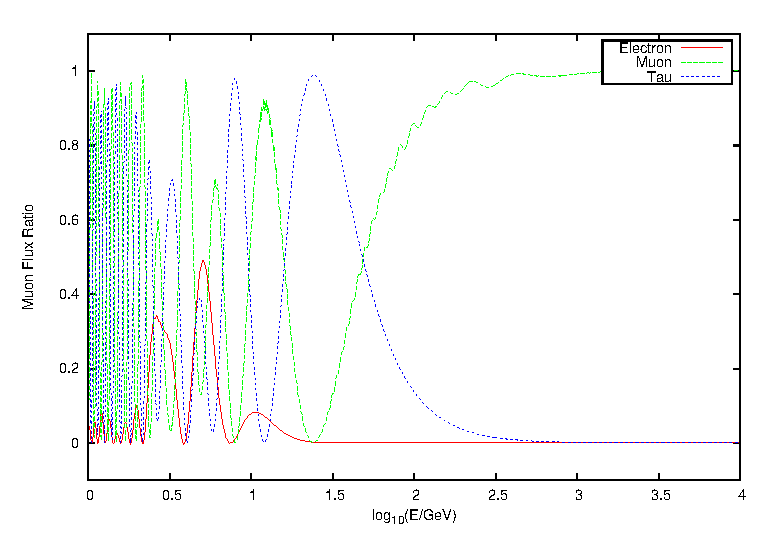
\includegraphics[width=0.7\textwidth]{fig/Multiplot.eps} 
  \caption{Output for the multiple energy mode with sterile neutrino (3+1)} 
\end{figure}
 
In fig.\ref{fig:multimode} we show the plot produced by the plotting
script for the case with sterile neutrino (3+1).


\subsection{Read and Write \textnormal{({\ttf examples/HDF5\_Write\_Read})}}

In this example we basically illustrate the use of the functions to
read and write {\ttf .hdf5} files. The content of the file is the full
information in the system, that means all the configuration
parameters, body, track, position in the track and also all the
density matrix information. This allows for example to save the system
in the middle of the propagation and read it later to keep
evolving. Another important fact is that if we save the system using
this when we read it again we can compute any quantum mechanical
observable for the saved density matrix.

This example is basically the same as the multiple energy example by
splited in two parts, one that computes the evolution ans save the
state of the system ({\ttf write.cpp}) and another that reads the
state and extract the flavor fluxes and put them in a text file ({\ttf
  read.cpp}).

In the following we will show the lines to save and load the hdf5
files.

In the file {\ttf write.cpp} we save the system before and after the
evolution.
\begin{lstlisting}[frame=leftline, numbers =
  left,breaklines=true,label = ex:sin1]
  nus.WriteStateHDF5(``./initial_state.hdf5'');
  nus.EvolveState();
  nus.WriteStateHDF5(``./final_state.hdf5'');
\end{lstlisting}

And in order to recover that in the {\ttf read.cpp} file we use the
constructor that construct directly the object for a given file name.

\begin{lstlisting}[frame=leftline, numbers =
  left,breaklines=true,label = ex:sin1]
  nuSQUIDS inus(``./initial_state.hdf5'');
  nuSQUIDS fnus(``./final_state.hdf5''); 
\end{lstlisting}


\subsection{Use and Construct Bodies \textnormal{({\ttf
      examples/Bodies})}}
One of the main classes in the nuSQUIDS library is the body and track
classes, these have to be always defined since they define the media
where the neutrinos will propagate. 
In this example we show how to use the objects already implemented in
the library and also how to create some objects from the classes
already defined.

In the folder {\ttf examples/Bodies/} the {\ttf main.cpp} file
contains the main function of the examples, that uses all the already
existing objects in nuSQUIDS and the example new modified object
defined in the heather and implementation files {\ttf exBody.h} and
{\ttf exBody.cpp}.

\subsubsection{Construct a derived Body}

Here is an example of hot to define a derived object for the EarthAtm
body, in this simple case the object is just an earth model with some
parameters that weight the relative densities in the different layers
of the earth, inner core, outer core, and mantel.

In order to implement that we have to be in the {\ttf nusquids} namespace and we define a
new class called {\ttf EarthMod} which is a derived class of {\ttf
  EarthAtm}, this means this new class we have all the properties,
values and function of the other class. 
\begin{lstlisting}[frame=leftline, numbers = left,breaklines=true,label = ex:sin1]

namespace nusquids{

class EarthMod: public EarthAtm{
public:
\end{lstlisting}
Here we define the main constructors that implement the changes,
basically we weight the inner core, outer core and mantle using the
values given by, {\ttf double frho1}, {\ttf double frho2}, {\ttf
  double frho3}
\begin{lstlisting}[frame=leftline, numbers = left,breaklines=true,label = ex:sin1,firstnumber=last]
  EarthMod(){}
  EarthMod(std::string earthmodel, double frho1, double frho2 , double
  frho3);
\end{lstlisting}
The function {\ttf Mod} allows to change the parameters ones the
object is already defined.
\begin{lstlisting}[frame=leftline, numbers =
  left,breaklines=true,label = ex:sin1,firstnumber=last]

  void  Mod(double frho1, double frho2, double frho3);
};

\end{lstlisting}

\subsubsection{Use of the Bodies}

In this part we will describe what is implemented in the {\ttf
  main.cpp} file.
This file defines a nuSQUIDS object and sets different bodies and
tracks, for everyone of these it evolve the system and shows the
probabilities in the screen.
For simplicity we use the single energy mode, \ref{sec:single}, but the use of the body
and track would be exactly the same for the multiple energy case.

First we construct the nuSQUIDS object for 3 neutrinos we set the
oscillation parameters and the energy of the neutrino that we
propagate.

\begin{lstlisting}[frame=leftline, numbers =
  left,breaklines=true,label = ex:sin1]
  nuSQUIDS nus(3,neutrino);
  nus.Set_MixingAngle(0,1,0.563942);
  nus.Set_MixingAngle(0,2,0.154085);
  nus.Set_MixingAngle(1,2,0.785398);
  nus.Set_SquareMassDifference(1,7.65e-05);
  nus.Set_SquareMassDifference(2,0.00247);
  nus.Set_CPPhase(0,2,0.0);

  squids::Const units;

  nus.Set_E(10.0*units.GeV);
\end{lstlisting}

\begin{enumerate}
\item {\ttf Earth}

The first example is the {\ttf Earth} body, in this case the track is
parametrized by the baseline of the experiment. Here we define the
body and track.
\begin{lstlisting}[frame=leftline, numbers =
  left,breaklines=true,label = ex:sin1,firstnumber=last]
  double baseline = 500.0*units.km;
  std::shared_ptr<Earth> earth = std::make_shared<Earth>();
  std::shared_ptr<Earth::Track> earth_track = std::make_shared<Earth::Track>(0.0,baseline,baseline);
\end{lstlisting}
And we set the Body and Track to the nusquids object.
\begin{lstlisting}[frame=leftline, numbers =
  left,breaklines=true,label = ex:sin1,firstnumber=last]
  nus.Set_Body(earth);
  nus.Set_Track(earth_track);
\end{lstlisting}

We first set the initial state of the system, and print the state in
the screen.
\begin{lstlisting}[frame=leftline, numbers =
  left,breaklines=true,label = ex:sin1,firstnumber=last]
  marray<double,1> ini_state({3},{0,1,0});
  nus.Set_initial_state(ini_state,flavor);
  // Lets print out the initial state
  std::cout << "In state" << std::endl;
  for (double EE : nus.GetERange()){
    std::cout << EE/units.GeV << " ";
    for(int i = 0; i < 3; i++){
      std::cout << nus.EvalFlavor(i) << " ";
    }
    std::cout << std::endl;
  }

We set the numerical error and maximum step for the GSL integrator.
\begin{lstlisting}[frame=leftline, numbers =
  left,breaklines=true,label = ex:sin1,firstnumber=last]
  nus.Set_h_max( 200.0*units.km );
  nus.Set_rel_error(1.0e-12);
  nus.Set_abs_error(1.0e-12);
\end{lstlisting}

Finally we evolve the state and print in the screen the final state of
the system.
\begin{lstlisting}[frame=leftline, numbers =
  left,breaklines=true,label = ex:sin1,firstnumber=last]

  nus.EvolveState();
  std::cout << "Out state" << std::endl;
  for (double EE : nus.GetERange()){
    std::cout << EE/units.GeV << " ";
    for(int i = 0; i < 3; i++){
      std::cout << nus.EvalFlavor(i) << " ";
    }
    std::cout << std::endl;
  }
\end{lstlisting}
This last steps in the code are the same in all the examples and we
are ommiting that for the following cases, we are only going to go though the
declaration of the body an track. 
\item {\ttf EarthAtm}

In this example we use the {\ttf EarthAtm} body. In this case the
track is defined by the zenith angle of the trajectory.
\begin{lstlisting}[frame=leftline, numbers =
  left,breaklines=true,label = ex:sin1,firstnumber=last]
  double phi = acos(-1.0);
  std::shared_ptr<EarthAtm> earth_atm = std::make_shared<EarthAtm>();
  std::shared_ptr<EarthAtm::Track> earth_atm_track = std::make_shared<EarthAtm::Track>(phi);

  nus.Set_Body(earth_atm);
  nus.Set_Track(earth_atm_track);
\end{lstlisting}

\item {\ttf earth\_mod}

Case with the modified earth object we construct as a derived object
of EarthAtm. As before the track is deffined by the zenith angle of
the trajectory, in this case we construct the object and then we rescale
all the earth density by a factor $0.1$, finally we set the body an track to nuSQUIDS. 
\begin{lstlisting}[frame=leftline, numbers =
  left,breaklines=true,label = ex:sin1,firstnumber=last]
  double phi = acos(-1.0);
  std::shared_ptr<EarthMod> earth_mod = std::make_shared<EarthMod>();
  std::shared_ptr<EarthMod::Track> earth_mod_track = std::make_shared<EarthMod::Track>(phi);  
  earth_mod->Mod(0.1,0.1,0.1);

  nus.Set_Body(earth_mod);
  nus.Set_Track(earth_mod_track);
\end{lstlisting}


\item {\ttf VariableDensity}

In this case we set a variable density body and a track of $200km$
First we define the density, position and electron fraction arrays
with the corresponding values.
\begin{lstlisting}[frame=leftline, numbers =
  left,breaklines=true,label = ex:sin1,firstnumber=last]
  int N=40;

  std::vector<double> x_arr(N);
  std::vector<double> density_arr(N);
  std::vector<double> ye_arr(N);

  double size = 1000.0*units.km;
  for(int i = 0; i < N; i++){
    x_arr[i] = size*(i/(double)N);
    density_arr[i] = fabs(cos((double)i));
    ye_arr[i] = fabs(sin((double)i));
  }
\end{lstlisting}

Now we construct the body and the track using, the constructor for the
variable density takes as an input the vectors with the
values. Finally like before we set the body ant the track to nuSQUIDS.
\begin{lstlisting}[frame=leftline, numbers =
  left,breaklines=true,label = ex:sin1,firstnumber=last]

  std::shared_ptr<VariableDensity> vardens = std::make_shared<VariableDensity>(x_arr,density_arr,ye_arr);
  std::shared_ptr<VariableDensity::Track> track_vardens = std::make_shared<VariableDensity::Track>(0.0,200.0*units.km);

  nus.Set_Body(vardens);
  nus.Set_Track(track_vardens);
\end{lstlisting}

\item {\ttf Vacuum}

This is a trivial case where the density and electron fraction are
zero, we only need to give the baseline as an argument to construct
the track. In the example we set the baseline to $500km$.

\begin{lstlisting}[frame=leftline, numbers =
  left,breaklines=true,label = ex:sin1,firstnumber=last]
  double baseline_2 = 500.0*units.km;
  std::shared_ptr<Vacuum> vacuum = std::make_shared<Vacuum>();
  std::shared_ptr<Vacuum::Track> track_vac = std::make_shared<Vacuum::Track>(baseline_2);
  
  nus.Set_Body(vacuum);
  nus.Set_Track(track_vac);
\end{lstlisting}

\item {\ttf ConstantDensity}

Case with constant density, in this case a analytic approximation is
used to propagate the neutrinos, the full Hamiltonian of the system is
diagonalized and exponentiated. This allows to solve very fast the
oscillations even when the matter potential is large.

We set the density to $100g/cm^3$ the electron fraction to 0.3 and the
baseline for the propagation to $500km$.
\begin{lstlisting}[frame=leftline, numbers =
  left,breaklines=true,label = ex:sin1,firstnumber=last]

  double density = 100.0;
  double ye = 0.3;
  std::shared_ptr<ConstantDensity> constdens = std::make_shared<ConstantDensity>(density,ye);
  double baseline_3 = 500.0*units.km;
  std::shared_ptr<ConstantDensity::Track> track_constdens =   std::make_shared<ConstantDensity::Track>(0.0,baseline_3);

  nus.Set_Body(constdens);
  nus.Set_Track(track_constdens);
\end{lstlisting}

Notice that the system sets the nusquids in the mass basis in order to
do the approximation, that can produce problems in the future uses of
the same nuSQUIDS object.

\end{enumerate}


\subsection{ Cross Sections \textnormal{({\ttf
      examples/Xsections})}}

One of the strong sides of nuSquids is the possibility of adding in a
consistent way the non coherent interaction, the physical quantity
that encodes how often this scattering interaction are happening
between the neutrinos and the media is the cross section and is all in
the cross section class.

In this example we show a very basic extension of the standard
cross section class in a way that extends the values to low energies, 
in the region where the cross section can be very well approximated by
zero.

The new derived class for the extended cross section is in the header
{\ttf exCross.h} and the implementation file {\ttf exCross.cpp}, the
main file is an example using this new cross section in the multiple
energy mode.

The new derived class {\ttf
  NeutrinoDISCrossSectionsFromTablesExtended} its just the same class
as {\ttf NeutrinoDISCrossSectionsFromTables} but returning zero for
the Total and differential cross sections when the energy is lower
than the lowest energy in the tables.

Here we define the constructor, the {\ttf TotalCrossSection} and {\ttf SingleDifferentialCrossSection}
\begin{lstlisting}[frame=leftline, numbers =
  left,breaklines=true,label = ex:sin1]
  
  class NeutrinoDISCrossSectionsFromTablesExtended : public NeutrinoDISCrossSectionsFromTables {
    public :
    NeutrinoDISCrossSectionsFromTablesExtended():NeutrinoDISCrossSectionsFromTables(){}
    double TotalCrossSection(double Enu, NeutrinoFlavor flavor, NeutrinoType neutype, Current current) const override;
    double SingleDifferentialCrossSection(double E1, double E2, NeutrinoFlavor flavor, NeutrinoType neutype, Current current) const override;
  };
 
\end{lstlisting}

The implementation file is just.
\begin{lstlisting}[frame=leftline, numbers =
  left,breaklines=true,label = ex:sin1]
  double NeutrinoDISCrossSectionsFromTablesExtended::TotalCrossSection(
  double Enu, NeutrinoFlavor flavor, NeutrinoType neutype, Current current) const{
    if (not (flavor == electron or flavor == muon or flavor == tau))
      return 0.0;
    if (Enu < Emin)
      return std::numeric_limits<double>::min();
    else
      return NeutrinoDISCrossSectionsFromTables::TotalCrossSection(Enu, flavor, neutype, current);
  }
  
  double NeutrinoDISCrossSectionsFromTablesExtended::SingleDifferentialCrossSection(double
  E1, double E2, NeutrinoFlavor flavor, NeutrinoType neutype, Current current) const{
    if (not (flavor == electron or flavor == muon or flavor == tau))
      return 0.0;
    if (E1 < Emin || E2<Emin)
      return std::numeric_limits<double>::min();
    else
      return NeutrinoDISCrossSectionsFromTables::SingleDifferentialCrossSection(E1, E2, flavor, neutype, current);
  }
 
\end{lstlisting}

In order to use that in the main function we construct the new cross
section object and construct the nusquids using that.

\begin{lstlisting}[frame=leftline, numbers =
  left,breaklines=true,label = ex:sin1]
  std::shared_ptr<NeutrinoCrossSections> ncs=std::make_shared<NeutrinoDISCrossSectionsFromTablesExtended>();
  nuSQUIDS nus(Emin,Emax,200,numneu,neutrino,true,true,ncs);
\end{lstlisting}


\begin{figure}[h!]
  \label{fig:crossext}
  \centering
  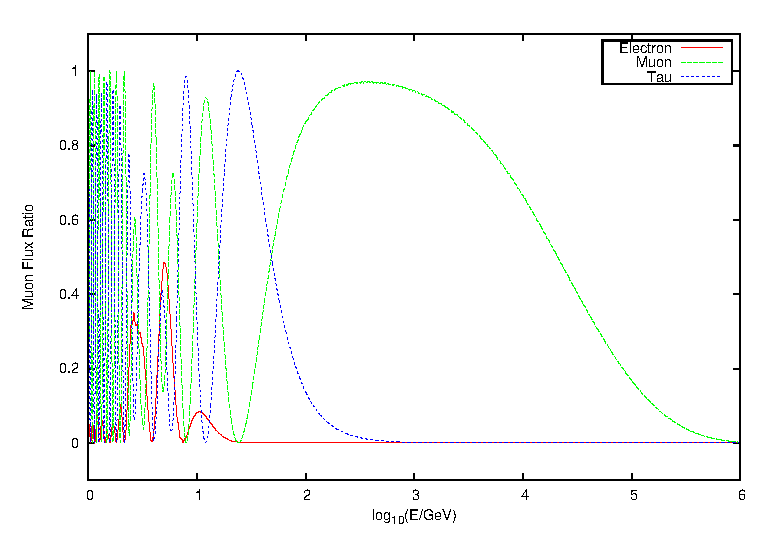
\includegraphics[width=0.7\textwidth]{fig/crossext.eps} 
  \caption{New low energy extended cross sections example} 
\end{figure}



\subsection{ Constant Density Layers \textnormal{({\ttf
      examples/Constant\_density\_layers})}}
Since the constant density allows us to do very fast computation using
the diagonalization of the full Hamiltonian here we show an example
where we concatenate the evolution of the neutrinos through different
layers of constant density.

First we construct the different layers, the first is $100km$ in
vacuum, the second $50km$ in matter with density $3.5g/cm^3$ and
$y_e=0.5$ and finally $200km$ in matter with density $10g/cm^3$ and
$y_e=0.1$.
\begin{lstlisting}[frame=leftline, numbers =
  left,breaklines=true,label = ex:sin1]

  const double layer_1 = 100.*units.km;
  std::shared_ptr<Vacuum> vacuum = std::make_shared<Vacuum>();
  std::shared_ptr<Vacuum::Track> track_env0 = std::make_shared<Vacuum::Track>(layer_1);

  const double layer_2 = 50.*units.km;
  std::shared_ptr<ConstantDensity> constdens_env1 = std::make_shared<ConstantDensity>(3.5,0.5); 
  std::shared_ptr<ConstantDensity::Track> track_env1 = std::make_shared<ConstantDensity::Track>(layer_2);

  const double layer_3 = 200.*units.km;
  std::shared_ptr<ConstantDensity> constdens_env2 = std::make_shared<ConstantDensity>(10.,0.1);
  std::shared_ptr<ConstantDensity::Track> track_env2 = std::make_shared<ConstantDensity::Track>(layer_3);

\end{lstlisting}

Now in order to evolve the system, we should set the corresponding body
and track and evolve every layer.
\begin{lstlisting}[frame=leftline, numbers =
  left,breaklines=true,label = ex:sin1]

  nus.Set_Body(vacuum);
  nus.Set_Track(track_env0);
  nus.EvolveState();


  nus.Set_Body(constdens_env1);
  nus.Set_Track(track_env1);
  nus.EvolveState();

  nus.Set_Body(constdens_env2);
  nus.Set_Track(track_env2);
  nus.EvolveState();

\end{lstlisting}

Finally we write the output for the different fluxes in flavor in a text file.

\subsection{ Non Standard Neutrino Interaction \textnormal{({\ttf
      examples/NSI})}}
Neutrino oscillations are a good probe for new physics, in this
example we illustrate an example of constructing a derived class of
nusquids in order to add some new physics modification, similarly can
be done in any other new physics scenario.

The implementation of the {\ttf nuSQUIDSNSI} is done in {\ttf NSI.h}.
First we will go trough the implementation to see what needs to be
added to be base class nuSQUIDS.
Some new variables are needed to implement the NSI matter potential,
We declare a {\ttf SU\_vector} called {\ttf NSI} that is the matter
potential, because we are working in the interaction picture we need
to define a matter potential that is accordingly rotated with $H_0$ for
every energy, this would be stored in {\ttf NSI\_evol}.
{\ttf HI\_prefactor} contains all the numerical factor in front of the
operator and {\ttf epsilon\_mutau} is the strength of the NSI non flavor
diagonal term, notice that we have the NSI diagonal contribution to
zero.

\begin{lstlisting}[frame=leftline, numbers =
  left,breaklines=true,label = ex:sin1]

class nuSQUIDSNSI: public nuSQUIDS {
  private:
    squids::SU_vector NSI;
    std::vector<squids::SU_vector> NSI_evol;
    std::unique_ptr<double[]> hiBuffer;
    double HI_prefactor;
    // nsi parameters
    double epsilon_mutau;

\end{lstlisting}

Before computing any derivative or r.h.s of the differential equation
we should have the NSI operator in the interaction picture. We add
this in prederive.
\begin{lstlisting}[frame=leftline, numbers =
  left,breaklines=true,label = ex:sin1,firstnumber=last]

    void AddToPreDerive(double x){
      for(int ei = 0; ei < ne; ei++){
        NSI_evol[ei] = NSI.Evolve(H0_array[ei],(x-Get_t_initial()));
      }
    }

\end{lstlisting}

This functions are auxiliary functions that allow the nuSQuIDSNSI to
save all the new information that defines the new derived object in
the hdf5 files.

\begin{lstlisting}[frame=leftline, numbers =
  left,breaklines=true,label = ex:sin1,firstnumber=last]

    void AddToReadHDF5(hid_t hdf5_loc_id){
      // here we read the new parameters now saved in the HDF5 file
      hid_t nsi = H5Gopen(hdf5_loc_id, "nsi", H5P_DEFAULT);
      H5LTget_attribute_double(hdf5_loc_id,"nsi","mu_tau" ,&epsilon_mutau);
      H5Gclose(nsi);
    }

    void AddToWriteHDF5(hid_t hdf5_loc_id) const {
      // here we write the new parameters to be saved in the HDF5 file
      H5Gcreate(hdf5_loc_id, "nsi", H5P_DEFAULT, H5P_DEFAULT, H5P_DEFAULT);
      H5LTset_attribute_double(hdf5_loc_id, "nsi","mu_tau",&epsilon_mutau, 1);
    }

\end{lstlisting}

And probably the most important part, where we compute the value of
the matter potential i.e. {\ttf HI}, notice at the end the different
sign for neutrinos and antineutrinos.
\begin{lstlisting}[frame=leftline, numbers =
  left,breaklines=true,label = ex:sin1,firstnumber=last]

    squids::SU_vector HI(unsigned int ei,unsigned int index_rho) const{
      double CC = HI_prefactor*body->density(*track)*body->ye(*track);


      squids::SU_vector potential(nsun,hiBuffer.get());

      potential = (3.0*CC)*NSI_evol[ei];

      if ((index_rho == 0 and NT==both) or NT==neutrino){
          return nuSQUIDS::HI(ei,index_rho) + potential;
      } else if ((index_rho == 1 and NT==both) or NT==antineutrino){
          return nuSQUIDS::HI(ei,index_rho) + (-1.0)*std::move(potential);
      } else{
          throw std::runtime_error("nuSQUIDS::HI : unknown particle or antiparticle");
      }
    }

\end{lstlisting}

In the public function we have the constructor, first calls the
nuSQUIDS constructor and after sets up the standard oscillation
paramters and the NSI operator.  
\begin{lstlisting}[frame=leftline, numbers =
  left,breaklines=true,label = ex:sin1,firstnumber=last]

  public:
  nuSQUIDSNSI(double epsilon_mutau, double Emin,double Emax,int Esize,int numneu, NeutrinoType NT,
	      bool elogscale,bool iinteraction,double th01=0.563942, double th02=0.154085, 
	      double th12=0.785398) : nuSQUIDS(Emin,Emax,Esize,numneu,NT,elogscale,iinteraction),
				      hiBuffer(new double[nsun*nsun]),epsilon_mutau(epsilon_mutau)
  {
    assert(numneu == 3);
    // defining a complex matrix M which will contain our flavor
    // violating flavor structure.
    gsl_matrix_complex * M = gsl_matrix_complex_calloc(3,3);
    gsl_complex c {{ epsilon_mutau , 0.0 }};
    gsl_matrix_complex_set(M,2,1,c);
    gsl_matrix_complex_set(M,1,2,gsl_complex_conjugate(c));
    
    NSI = squids::SU_vector(M);
    
    Set_MixingAngle(0,1,th01);
    Set_MixingAngle(0,2,th02);
    Set_MixingAngle(1,2,th12);
    
    // rotate to mass reprentation
    NSI.RotateToB1(params);
    NSI_evol.resize(ne);
    for(int ei = 0; ei < ne; ei++){
      NSI_evol[ei] = squids::SU_vector(nsun);
    }
    gsl_matrix_complex_free(M);
    
    HI_prefactor = params.sqrt2*params.GF*params.Na*pow(params.cm,-3);
  }

\end{lstlisting}

This last function set the value of {\ttf epsilon\_mutau}, changing the
value of the {\ttf SU\_vector NSI} accordingly 

\begin{lstlisting}[frame=leftline, numbers =
  left,breaklines=true,label = ex:sin1,firstnumber=last]
  
  void Set_mutau(double eps){
    gsl_matrix_complex * M = gsl_matrix_complex_calloc(3,3);
    gsl_complex c {{ epsilon_mutau , 0.0 }};
    gsl_matrix_complex_set(M,2,1,c);
    gsl_matrix_complex_set(M,1,2,gsl_complex_conjugate(c));
    NSI = squids::SU_vector(M);    
    NSI.RotateToB1(params);
    gsl_matrix_complex_free(M);
  }
 
  
\end{lstlisting}


In the main function in {\ttf main.cpp} we use the new NSI in a
multiple energy mode. In order
to see the effect of having NSI we propagate the case with {\ttf
  epsilon\_mutau=0} and {\ttf epsilon\_mutau=1e-2}.


\begin{lstlisting}[frame=leftline, numbers =
  left,breaklines=true,label = ex:sin1,firstnumber=last]

  double eps_mutau=1.0e-2;
  nuSQUIDSNSI nus(eps_mutau,Emin,Emax,200,numneu,antineutrino,true,false);
  nuSQUIDSNSI nus_zero(0.0,Emin,Emax,200,numneu,antineutrino,true,false);
\end{lstlisting}

After setting all the parameters we propagate both cases, and put both
fluxes in a text file.

\begin{lstlisting}[frame=leftline, numbers =
  left,breaklines=true,label = ex:sin1,firstnumber=last]

  nus.EvolveState();
  nus_zero.EvolveState();

  int Nen =1000;
  double lEmin=log10(Emin);
  double lEmax=log10(Emax);
  
  std::ofstream file("fluxes_flavor.txt");

  file << "# log10(E) E flux_NSI_i flux_noNSI_i . . . ." << std::endl;
  for(double lE=lEmin; lE<lEmax; lE+=(lEmax-lEmin)/(double)Nen){
    double E=pow(10.0,lE);
    file << lE << " " << E << " ";
    for(int fl=0; fl<numneu; fl++){
      file << " " <<  nus.EvalFlavor(fl, E) << " " <<  nus_zero.EvalFlavor(fl, E);
    }
    file << std::endl;
  }

\end{lstlisting}

In the folder there is a script that allows to plot the output text
file.

\subsection{ Atmospheric Mode \textnormal{({\ttf
      examples/Atm\_default})}}
In this example we show how to use the atmospheric mode, this mode is
compact way to treat set of nuSQUIDS objects distributed in zenith, this
allows us to treat the problem of
propagating the full, energy and zenith dependent, atmospheric neutrino flux trough the earth.

First we construct the nuSQUIDSAtm object. The paremeters we are
setting is the range of cosine of the zenith angle from $-1$ to $0.2$
and in energies from $10GeV$ to $1e6GeV$, we chose 40 nodes in zenith.
Notice that the parameters after the zenith information are the same
than the basic nuSQUIDS object.

\begin{lstlisting}[frame=leftline, numbers =
  left,breaklines=true,label = ex:sin1]

  double Emin=1.e1*units.GeV;
  double Emax=1.e6*units.GeV;
  double czmin=-1;
  double czmax=0;

  nuSQUIDSAtm<> nus_atm(czmin,czmax,40,Emin,Emax,100,numneu,both,true,interactions);

\end{lstlisting}

In this case we have to give the initial state also depending on
zenith, here we fill the array with and set the initial state of the
system. The function {\ttf flux\_function} would be the corresponding
atmospheric flux.

\begin{lstlisting}[frame=leftline, numbers =
  left,breaklines=true,label = ex:sin1,firstnumber=last]

  marray<double,4> inistate{nus_atm.GetNumCos(),nus_atm.GetNumE(),2,numneu};
  std::fill(inistate.begin(),inistate.end(),0);
  for ( int ci = 0 ; ci < nus_atm.GetNumCos(); ci++){
    for ( int ei = 0 ; ei < nus_atm.GetNumE(); ei++){
      for ( int rho = 0; rho < 2; rho ++ ){
        for (int flv = 0; flv < numneu; flv++){
          inistate[ci][ei][rho][flv] = (flv == 1) ? flux_function(e_range[ei], cz_range[ci]) : 0.0;//set 1 only to the muon flavor
        }
      }
    }
  }

  nus_atm.Set_initial_state(inistate,flavor);

\end{lstlisting}


To evolve the full state we call

\begin{lstlisting}[frame=leftline, numbers =
  left,breaklines=true,label = ex:sin1,firstnumber=last]

nus_atm.EvolveState();

\end{lstlisting}

Finally we save the flux in a output text file, notice that the
atmospheric mode has an interpolation implemented, therefore you can
evaluate the flux at any flavor, energy, and zenith. See \ref{sec:atm}
for more details.
\ref{sec:atm}.

\begin{lstlisting}[frame=leftline, numbers =
  left,breaklines=true,label = ex:sin1,firstnumber=last]

  int Nen=700;
  int Ncz=100;
  double lEmin=log10(Emin);
  double lEmax=log10(Emax);;

  file << "# log10(E) cos(zenith) E flux_i . . . ." << std::endl;
  for(double cz=czmin;cz<czmax;cz+=(czmax-czmin)/(double)Ncz){
    for(double lE=lEmin; lE<lEmax; lE+=(lEmax-lEmin)/(double)Nen){
      double E=pow(10.0,lE);
      file << lE << " " << cz << " " << E;
      for(int fl=0; fl<numneu; fl++){
	file << " " <<  nus_atm.EvalFlavor(fl,cz, E);
      }
      file << std::endl;
    }
    file << std::endl;
  }

\end{lstlisting}



\subsection{ Atmospheric With Derived nuSQUIDS Class \textnormal{({\ttf
      examples/Atm\_NSI})}}

The Atmospheric mode is done in a way that can be used not only with
the basic nuSQUIDS class but also with derived classes. In this
example we use the atmospheric mode but with the NSI nuSQUIDS
extension shown in the NSI example.

In the folder we add the {\ttf NSI.h} file, this file is exactly the
same as in the NSI example, and the main file is essentially the same as
the atmospheric default mode example with the following changes.

\begin{lstlisting}[frame=leftline, numbers =
  left,breaklines=true,label = ex:sin1,firstnumber=last]

  double epsilon_mutau=1e-2;
  nuSQUIDSAtm<nuSQUIDSNSI> nus_atm(czmin,czmax,40,epsilon_mutau,Emin,Emax,100,numneu,both,true,true);

\end{lstlisting}

notice that in this example the arguments are always, first the zenith
arguments {\ttf czmin, czmax, 40} and second the arguments of the
nuSQUIDS derive object, in this case for the NSI {\ttf
  epsilon\_mutau,Emin,Emax,100,numneu,both,true,true}. This structure
will hold for any derive nuSQUIDS class.


 